\section{The \textit{housemodel} Python package}

\subsection{Cloning from Github}

The Git repository with the HAN housemodel is located in the cloud, on the GitHub site. The URL is:

\url{https://github.com/hancse/twozone_housemodel}

The repository contains a Python package \emph{housemodel}. The Python package is actively updated and upgraded.

Currently, the repository is \emph{public}. 
This means you do not need a GitHub account for read access permission to download or clone the repository. 
For contributing, write permission needs to be granted by the administrator(s). In order to obtain a GitHub account, follow the instructions in Appendix \ref{appendix::account}.

%If permissions are granted, proceed with one of the options below:

\subsubsection{Option 1}
\begin{itemize}
	\item this option generates a folder with the latest code version for \emph{users}. Contributing is not possible because the \textsf{.git} folder (repository bookkeeping) is not included in the download. 
	\item Follow the link above to the cloud repository.
	\item Click the button with "\textbf{...}" and select "Download repository".
	\item The downloaded zip archive is named "twozone-housemodel-xxxxxxxxxxxx.zip" Unpack the folder in the zip archive. The xxxxxxxxxxxx code indicates the unique commit (version) number of the downloaded code. Do not change the name of the downloaded and unpacked folder.
\end{itemize}

\subsubsection{Option 2}

\begin{itemize}
	\item this option generates a \emph{local} clone with the complete history of the repository in the \textsf{.git} folder. This is for programmers and contributing \emph{users}. Contributors must be aware of the workflow mentioned in Appendix \ref{appendix:workflow}.
    \item Follow the instructions in Appendix \ref{appendix:versioning}. 
    \item Read the notes in Appendix \ref{appendix::gitnotes}
	\item make a new \emph{local} folder on your HDD or SSD disk and name it \textsf{"housemodel-git"}.
	\item go to the (empty) folder and click the right mouse button to open the context menu of Fig.~\ref{fig:Tortoise_context}.
	\item choose the menu option \textsf{"Git clone..."}.The dialog from Fig.~\ref{fig:clone} appears.
	\item fill the entry \textsf{"URL:"} with the internet address (URL) of the repository above.
	\item fill the entry: \textsf{"Directory:"} with the path to your new local folder. A dummy name with placeholders $\langle username \rangle$ and $\langle programs \rangle$ is given in Fig.~\ref{fig:clone}. 
	\item leave all checkboxes unchecked.
	\item Press the OK button.
	\item A dialog with an acrobatic turtle will appear. The dialog will prompt you for your Bitbucket username and password. It will print a "Success" message when cloning has been completed.
\end{itemize}

\begin{figure}[H]
	\centering
	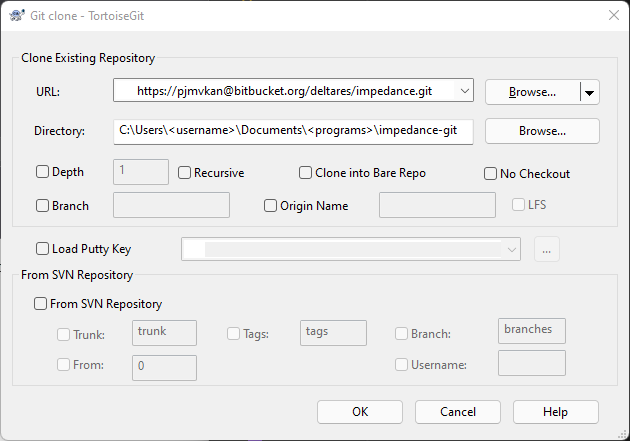
\includegraphics[width=0.6\textwidth]{Figures/Tortoise_clone_impedance}
	\caption{Cloning a repository with TortoiseGit}
	\label{fig:clone}
\end{figure}

\textit{Note}: Running the simulations and tests is best done from the \emph{repository root}. All simulations and tests are designed to find the package, subpackages and configuration files from this directory.

\subsection{Working with the Python code}

Python scripts and programs can only be run by the Python \emph{interpreter}. Installation of this interpreter and other Python \emph{packages} for mathematical operations, basic plotting and file handling, is done by a \emph{package manager} who bundles the packages in an \emph{environment}.

To get things working, follow the instructions in Appendix \ref{appendix:second}.

\begin{itemize}
	\item The commands for creating a dedicated \emph{environment} in Appendix \ref{appendix:config} and \ref{appendix:environments} are listed in Listing \ref{list:impenv}.
\end{itemize}

\lstinputlisting[label=list:impenv,caption=Example textfile with conda commands for new environment, language=Python, linerange={1-100}]{../../environment.txt}

\begin{itemize}
	\item after completion of the dedicated \emph{environment} the Python scripts in the folder "\textsf{twozone\_housemodel-xxxxxxxxxxxx}" or "\textsf{housemodel-git}" can be run in the \textsf{Anaconda Prompt} console.
	\item Alternatively, Python scripts can be run and adapted in an "Integrated development Environment (IDE). The recommended choice is the PyCharm IDE. For installation instructions, follow Appendix \ref{appendix:ide}.
\end{itemize}

\subsection{Package structure}

The repository "\textsf{twozone\_housemodel-git}" contains the modules for the house model. The customary way to organize the modules is to make a \emph{Python package} with \emph{subpackages}. This opens up the possibility of publishing the package on PyPi, so that it can be imported.

See: \url{https://pypi.org/}

From commit \textsf{e74ce58} the files in the \textsf{twozone\_housemodel-git} repository are organized as a package. The proposed structure, implemented in this commit, is:

\dirtree{%
	.1 twozone\_housemodel-git.
	.2 /Documentation.
	.3 /Reference\_Manual.
	.4 \textit{house\_model\_reference\_manual.tex}.
	.4 /Figures.
	.4 /Listings.
	.4 /pdf.
	.5 \textit{this document}.
	.2 \textit{housemodel}.
	.3 \_\_init\_\_.py.
	.3 /basics.
	.4 \_\_init\_\_.py.
	.4 ckf\_tools.py.
	.4 components.py.
	.4 flows.py.
	.4 source\_term.py.
	.4 totalsystem.py.
    .3 /buildings.
	.4 \_\_init\_\_.py.
	.4 building.py.
	.3 controls.
	.4 \_\_init\_\_.py.
	.4 heating\_curves.py.
	.4 Temperature\_SP.py.
	.4 /ivPID.
	.5 PID.py.
	.3 solvers.
	.4 \_\_init\_\_.py.
	.3 sourcesink.
	.4 \_\_init\_\_.py.
	.4 /buffervessels.
	.4 /heatpumps.
	.4 /radiators.
	.3 tools.
	.4 \_\_init\_\_.py.
	.2 tests.
	.3 \_\_init\_\_.py.
	.3 context1.py.
	.3 test\_*.py.
	.2 environment.txt.
	.2 Simulation*.py.
	.2 README.
	.2 setup.py (to be added).
} 

\begin{itemize}
	\item the \emph{repository root} \textsf{twozone\_housemodel-git} contains the simulation scripts and configuration files (for now) 
	\item the \emph{package root} \textsf{housemodel} contains the complete package. This can be seen since it contains an (empty) \textsf{\_\_init\_\_.py} module.
	\item the \emph{subpackage} folders contain the modules with common functions and classes for all simulations. They each contain an (empty) \textsf{\_\_init\_\_.py} module.
	\item a \textsf{tests} folder is placed carefully as a subfolder of the \emph{repository root}. 
	See: \url{https://docs.python-guide.org/writing/structure/} for the underlying philosophy. Here, testing modules (scripts) can be placed. If the names of the test scripts start with \textsf{test\_}, they can be automatically run with the \textsf{pytest} Python package.
\end{itemize}

\textit{Note}: Running the simulations and tests is best done from the \emph{repository root}. All simulations and tests have been updated to find the package, subpackages and configuration files from this directory.

\subsubsection{Subpackage \textsf{classes}}
 The subpackage \textsf{classes} contains the following Python modules:

 \begin{itemize}
	\item \textbf{constants.py}. This module contains basic physical constants listed in Listing~\ref{list:constants}.
\end{itemize}

% \lstinputlisting[label=list:constants,caption= Physical Constants in 
% constants.py, language=Python, linerange={2-11}]{Listings/constants.py}
 
 \begin{itemize}
     \item \textbf{cells.py}. This module covers Python classes for describing the electrolysis cells used in the experiments and simulations. The (abstract) base class \textsf{Cell} has an attribute \textsf{cell\_constant}. Derived classes \textsf{PlanarCell} and \textsf{CylindricalCell} contain specific geometrical parameters used for determining the frequency dependence of electrode polarization. See Listing~\ref{list:cells}.
 \end{itemize}
 
% \lstinputlisting[label=list:cells,caption= Class Cell and derived classes in 
% cells.py, language=Python, linerange={2-49}]{Listings/cells.py}

 \begin{itemize}
     \item \textbf{electrolytes.py}. This module covers Python classes for describing the basic electrolytes (ionic salt solutions) used in the experiments and simulations. The base class \textsf{Electrolyte} contains the attributes and methods listed in Listing~\ref{list:electrolytes}.
 \end{itemize}
 
% \lstinputlisting[label=list:electrolytes,caption= Class Electrolyte in
% electrolytes.py, language=Python, linerange={2-61}]{Listings/electrolytes.py}

 \begin{itemize}
     \item \textbf{particles.py}. This module covers Python classes for describing the colloidal particles present in the ionic solutions. The base class \textsf{Particles} contains the attributes and methods listed in Listing~\ref{list:particles}.
 \end{itemize}
 
% \lstinputlisting[label=list:particles,caption= Class Particles in particles.py,
% language=Python, linerange={2-35}]{Listings/particles.py}

 \begin{itemize}
     \item \textbf{colloids.py}. This module covers Python classes for describing the colloidal systems consisting of a cell, an electrolyte and colloidal particles. The base class \textsf{Colloids} contains the attributes and methods listed in Listing~\ref{list:colloids}.
 \end{itemize}
 
% \lstinputlisting[label=list:colloids,caption= Class Colloids in colloids.py,
% language=Python, linerange={2-60}]{Listings/colloids.py}

\subsection{Use Case}

 \begin{itemize}
	\item \textbf{import classes}
\end{itemize}

% \lstinputlisting[label=list:import, caption=, language=Python,
% linerange={11-16}]{Listings/testloadshort10mM_object_oriented.py}

 \begin{itemize}
	\item \textbf{instantiate classes}
\end{itemize}

% \lstinputlisting[label=list:instantiate, caption=, language=Python,
% linerange={53-58}]{Listings/testloadshort10mM_object_oriented.py}

 \begin{itemize}
	\item \textbf{perform calculations}
\end{itemize}

% \lstinputlisting[label=list:calculations, caption=, language=Python,
% linerange={60-67}]{Listings/testloadshort10mM_object_oriented.py}

 \begin{itemize}
	\item \textbf{load-short correction}
\end{itemize}

% \lstinputlisting[label=list:loadshort, caption=, language=Python,
% linerange={73-74}]{Listings/testloadshort10mM_object_oriented.py}

 \begin{itemize}
	\item \textbf{equivalent circuit}
\end{itemize}

% \lstinputlisting[label=list:eq_circ, caption=, language=Python, 
% linerange={69-71}]{Listings/testloadshort10mM_object_oriented.py}

\subsection{Stratified Buffer Vessel}

The \textsf{StratifiedBuffer} class in the module \textsf{stratified.py} contains the representation of a stratified buffer vessel. The vessel is assumed to have a \emph{cylindrical} shape. Therefore it has the following attributes:

\begin{itemize}
	\item (input) volume $V$ in $m$.
	\item (input) height $h$ in $m$
	\item (input) num\_layers $N$
	\item {layer\_height = $h / N$}
	\item radius $r = \sqrt{[V / (h * \pi)]}$
	\item wall surface of a layer $A_{wall,layer} = 2 * \pi * r * h/N$
	\item $A_{base} = V / h = \pi * r^2$
	\item cap\_layer = $(V / N) * \rho * c_p$
\end{itemize}

\lstinputlisting[label=list:stratified, caption=, language=Python, linerange={178-224}]{../../housemodel/sourcesink/buffervessels/stratified.py}

The \textsf{StratifiedBuffer} class is a central component in the thermal network. Therefore, the class shares the attributes:
\begin{itemize}
	\item \textsf{nodes} of type \textsf{CapacityNode}. \textsf{num\_nodes} equals num\_layers $N$.
	\item \textsf{edges} of type \textsf{CondEdge}. \textsf{num\_edges} equals $N-1$.
	\item a boundary condition \textsf{ambient} representing the indoor surroundings of the buffer vessel.
\end{itemize}

In contrast to the other \textsf{housemodel} classes, the internal capacitive nodes, conductive edges and ambient node, and hence the $\mathbf{C^{-1}}$, $\mathbf{K_{int}}$ and $\mathbf{K_{ext}}$-matrices can be calculated from the input parameters and need not be read from the configuration file. For this purpose the following methods are added to this class:

\begin{itemize}
	\item \textsf{generate\_nodes}
	\item \textsf{generate\_edges}
	\item \textsf{generate\_ambient}
\end{itemize}

The attributes \textsf{begin\_node} and \textsf{end\_node} = \textsf{begin\_node + n\_layers-1} are added to provide the anchor point(s) to the house model.


\newpage
